%!TEX root = booklet.tex

\section{SIGMOD Banquet (sponsored by Facebook)}

\begin{figure*}[h]
\centering

\includegraphics[width=.5\textwidth]{images/noorderlicht.jpg}
\end{figure*}

For this year's SIGMOD we have organized something different: The dinner will take place outdoors in a festival-like atmosphere in the post-industrial setting of the former shipyards of Amsterdam-North. Though only 15 minutes away from Central Station, the NDSM-yard is an open space for serenity, creativitiy and festivities all throughout the year.

With a magnificent backdrop of the river "IJ", our dinner location "Noorderlicht" is a well-known counter-culture location for hanging out with friends, having a drink and listening to music. We trust the relaxed atmosphere there will rub off on SIGMOD attendants. We will serve locally sourced and produced food and beverages from several food trucks. There will be tents, barbecue, fire places and more. We do have a plan B for if it should rain unexpectedly.

Hereby we would like to thank Facebook for sponsoring this event.

\begin{figure*}[h]
\centering
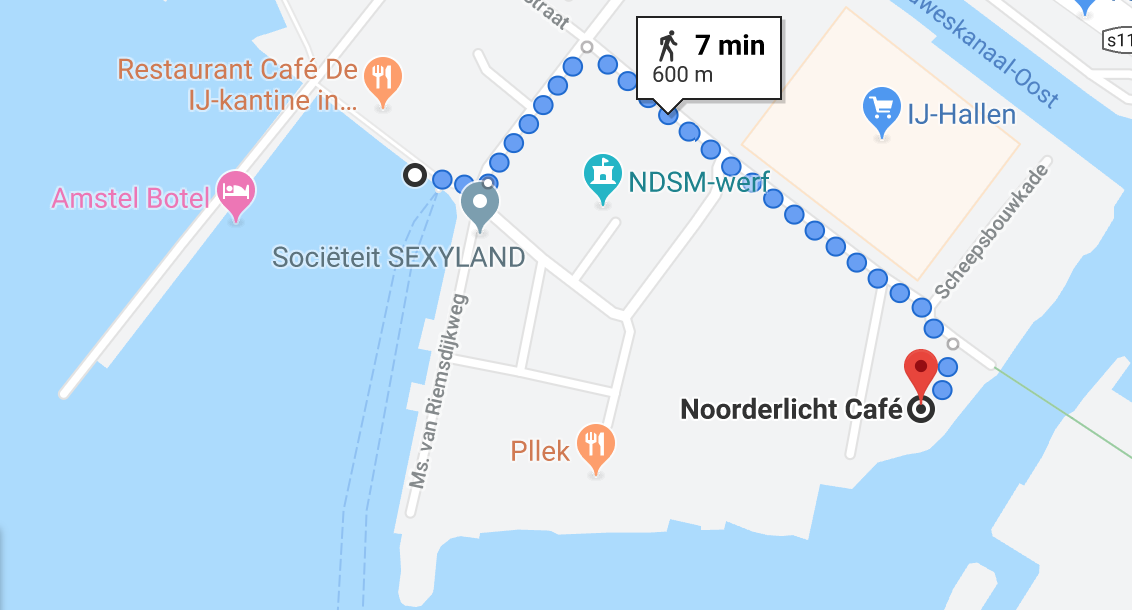
\includegraphics[width=.7\textwidth]{images/berlage-stromma.png}

Beurs van Berlage $\rightarrow$ Stromma jetties
\end{figure*}

Attendants will be transferred to Noorderlicht by way of a canal cruise passing through the UNESCO world heritage canals of historic Amsterdam. The cruise will leave close by the conference venue (at the Stromma jetties, close by the venue on your right-hand side when exiting it) and will take ca.\ one hour. The cruise concludes right in front of the dinner location. Everybody will be assigned a time slot ticket for the start of their cruise, please keep to your assigned time, or swap tickets with somebody else.

\begin{figure*}[h]
\centering
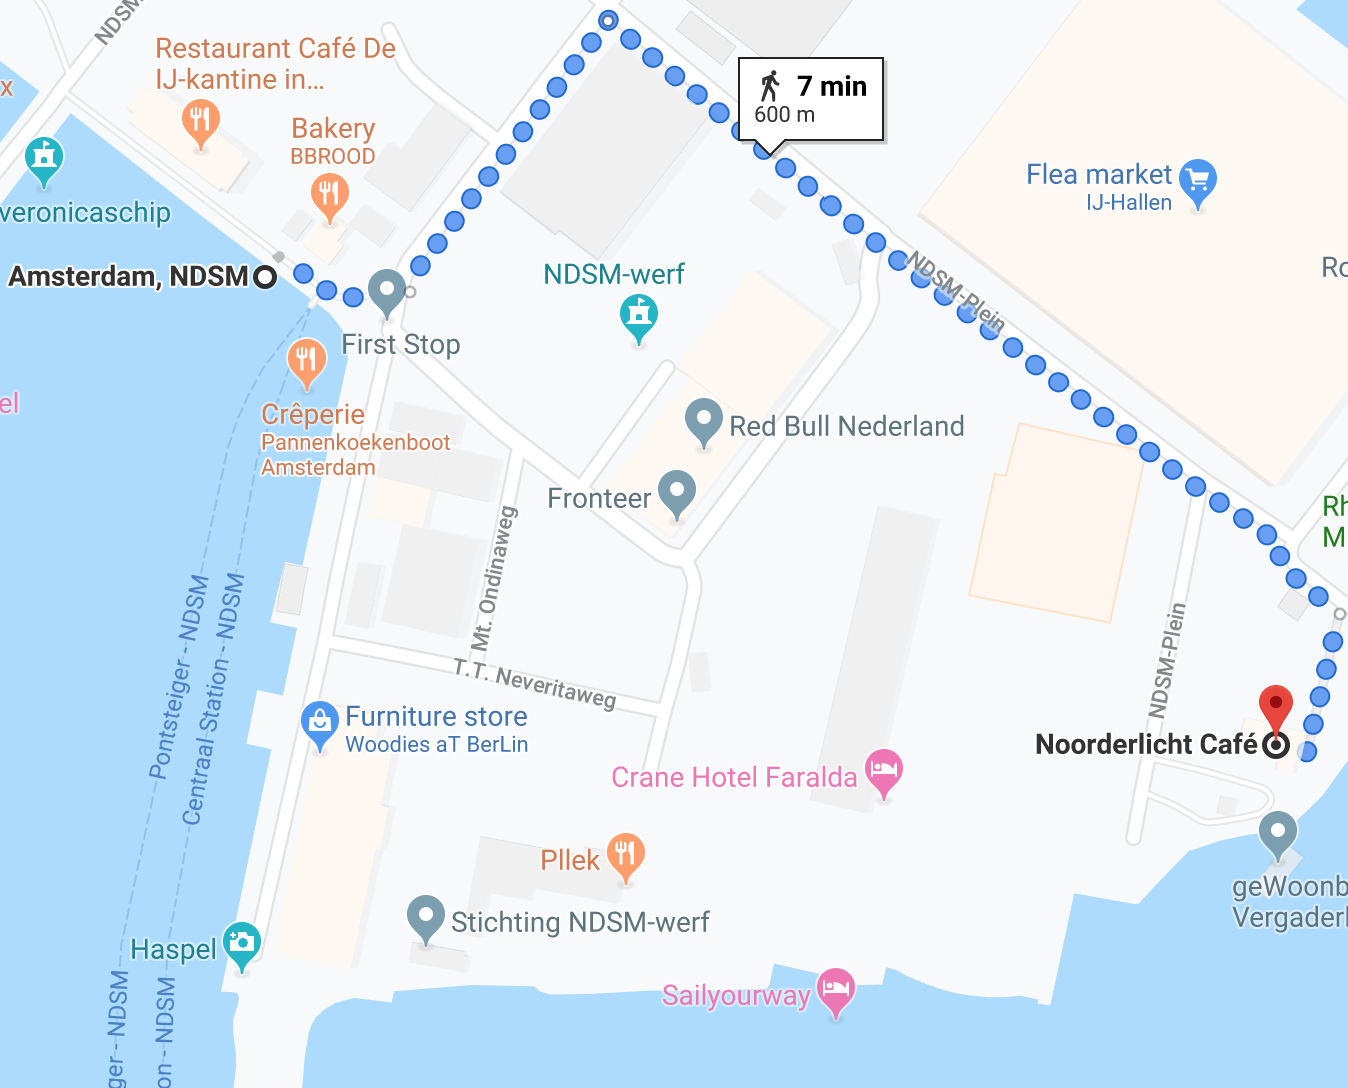
\includegraphics[width=.7\textwidth]{images/noorderlicht-ndsmferry.png}

Noordelicht Cafe $\rightarrow$ ferry terminal
\end{figure*}


For the way back to the city center, we will take the free municipal ferry service back to central station, with the last ferry leaving at midnight. The ferry terminal is a short (400m) walk away from Noorderlicht.
